\documentclass[a4]{beamer}
\usepackage{amssymb}
\usepackage{graphicx}
\usepackage{subfigure}
\usepackage{newlfont}
\usepackage{amsmath,amsthm,amsfonts}
%\usepackage{beamerthemesplit}
\usepackage{pgf,pgfarrows,pgfnodes,pgfautomata,pgfheaps,pgfshade}
\usepackage{mathptmx}  % Font Family
\usepackage{helvet}   % Font Family
\usepackage{color}

\mode<presentation> {
 \usetheme{Default} % was Frankfurt
 \useinnertheme{rounded}
 \useoutertheme{infolines}
 \usefonttheme{serif}
 %\usecolortheme{wolverine}
% \usecolortheme{rose}
\usefonttheme{structurebold}
}

\setbeamercovered{dynamic}

\title[MA4704]{Technological Mathematics 4 \\ {\normalsize MA4704 Lecture 12C}}
\author[Kevin O'Brien]{Kevin O'Brien \\ {\scriptsize Kevin.obrien@ul.ie}}
\date{Spring Semester 2013}
\institute[Maths \& Stats]{Dept. of Mathematics \& Statistics, \\ University \textit{of} Limerick}

\renewcommand{\arraystretch}{1.5}

\begin{document}

\begin{frame}
\titlepage
\end{frame}

\begin{frame}
\begin{itemize}
\item Consider two populations X and Y that are indepedently distributed from
each other.
\item That is to say, the true value of correlation is zero.
\[\rho_{XY} = 0 \]
\item In the context of a linear regression model, in the form $Y=\beta_0  +  \beta_1X$, a true correlation value of zero is equivalent to a true slope value of Zero.
\["\rho_{XY} = 0" \rightarrow\leftarrow "\beta_1=0"\]
\end{itemize}
\end{frame}
%----------------------------------------%
\begin{frame}
\frametitle{Random Samples}
\begin{itemize}
\item Consider two random samples drawn from X and Y respectively.
\item When these observations are plotted on a scatterplot, it
may be the case that some sort of relationship \textbf{appears} to exist (when in fact it doesn't).
\item The smaller the number of observations, the more likely this erroneous conclusion will occur.
\end{itemize}
\end{frame}
%-------------------------------------------%
\begin{frame}
\frametitle{Hypothesis Testing}
\begin{itemize}
\item To guard against making erroneous conclusions, a hypothesis test on the slope regression coefficient is
recommended.
\item The null hypothesis expresses the conservative viewpoint that no linear relationship between X and Y exists, and that the true value of the slope is zero.
\item The alternative hypothesis is that there is a linear relationship between X and Y, and that the slope is not zero.
\end{itemize}
\begin{eqnarray}
\mbox{H}_{0} : \beta_1 = 0 \\
\mbox{H}_{1} : \beta_1 \neq 0 \\
\end{eqnarray}
Remember to describe the hypotheses in your answers.
\end{frame}
%-------------------------------------------%
\begin{frame}
\frametitle{Regression: Hypothesis Testing}
\begin{itemize}
\item The test statistic for this test follows the general form of all test statistics.
\item The observed value is the slope estimate $b_1$ derived from the Least Squares estimation.
\item The expected value under the null hypothesis is 0.
\item The standard error is a complex two step calculation. (Formulae given in exam paper).
\end{itemize}
\end{frame}
%-------------------------------------------%
\begin{frame}
\frametitle{Regression: Hypothesis Testing}
\begin{figure}
  % Requires \usepackage{graphicx}
  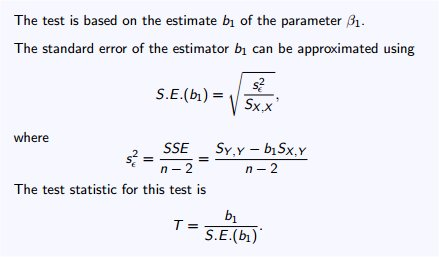
\includegraphics[scale=0.7]{TestStat.jpg}\\
\end{figure}
\end{frame}
%-------------------------------------------%
\begin{frame}
\frametitle{Regression: Hypothesis Testing}
\begin{itemize}
\item If the assumptions of the regression model are satisfied, this
statistic has a Student t-distribution with n - 2 degrees of freedom.
\item For large n this is approximately standard normal.
\item The critical value for this test is $t_{(n-2,\alpha/2)}$
\item This is the same procedures as for the previous section, but with $n-2$ degrees of freedom, rather than $n-1$).
\end{itemize}
\end{frame}
%-------------------------------------------%
\begin{frame}
\frametitle{Regression: Hypothesis Testing}
It should be noted that this test is not useful for detecting
non-monotonic (i.e. certain non-linear) dependencies (for example,
the quadratic like relationship plotted as one of the examples at
the beginning of the chapter)
\end{frame}
%-------------------------------------------%
\end{document}